\begin{optimproblem}{Basic cylindrical junction ($\dot{\gamma}^{A}_{\text{nw}}$)}
	\vspace{2mm}
	Objective:  Minimizing near-wall shear rate $\dot{\gamma}^{A}_{\text{nw}}$.
	
	\vspace{2mm}
	Geometrical model:
	\begin{itemize}
		\item Model 1 as described in Section~\ref{mod:model1}.
		\item Optimization parameters: offset $o_1$.
	\end{itemize}
	Constraints:
	\begin{itemize}
		\item Offset constraint: $0{,}0~\text{cm} \leq o_1 \leq 2{,}4~\text{cm}$.
		\item Flow split constraint: $F^{\text{LPA}}_{\text{IVC}} \geq 25~\%$.
	\end{itemize}
	Optimization method:
	\begin{itemize}
		\item Nelder-Mead method as described in Section~\ref{framework} and Appendix~\ref{appendix C}.
	\end{itemize}
	Initial point: $o^{\text{init}}_{1}$ = 0{,}39 cm
	\label{optimprob:1}
\end{optimproblem}

\begin{figure}[H]
	\centering
	\begin{subfigure}{0.47\textwidth}
		\centering
		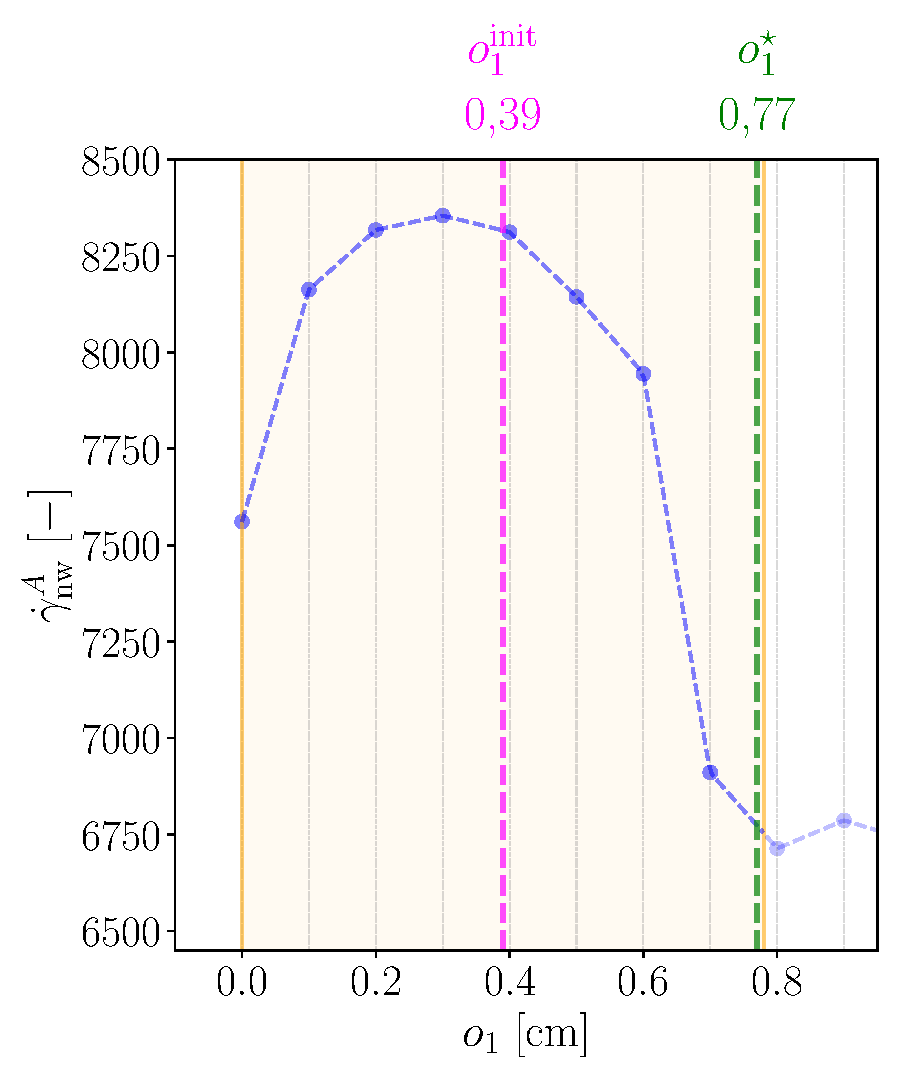
\includegraphics[
		width=\textwidth,
		trim={0mm 0mm 0mm -23mm}, clip
		]{figures/mean_stress_3_interpolated_point.pdf}
	\end{subfigure}\hfill%
	\begin{subfigure}{0.52\textwidth}
		\centering
		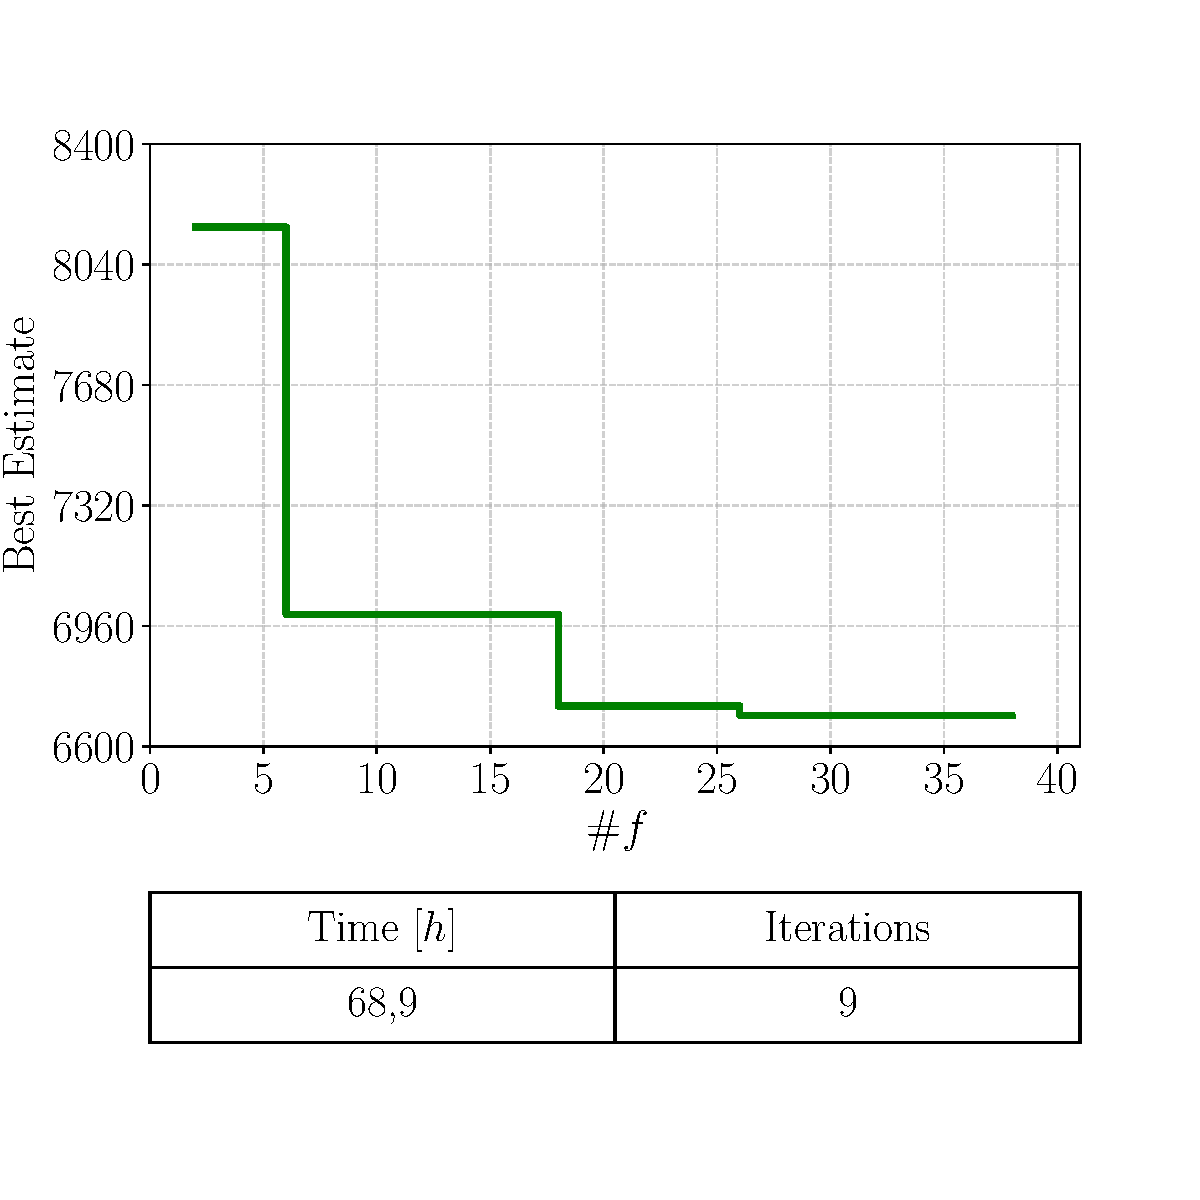
\includegraphics[
		width=1.05\textwidth,
		trim={0mm 25mm 0mm 0mm}, clip
		]{figures/optim_results/nm_sr.pdf}
	\end{subfigure}
	\vspace{2mm}
	\caption{Optimization results for Optimization Setup 1. The left plot compares the optimization result (marked point) with the previously sampled and interpolated objective function $\dot{\gamma}_{\text{max}}^{A}$ as a function of the parameter $o_1$. The right plot demonstrates the convergence of the optimization method, showing the best estimate against the number of objective function evaluations ($\# f$). The table summarizes the total elapsed time of the optimization algorithm (68,9 hours) and the number of iterations of the used method (9).}
\end{figure}
\newpage